
\textcolor{blue}{\textit{Philippe CHUZEL}}

The code which have been implemented for this part of the project can be sum up with the following picture \ref{fig:SyntheseCodeRegulationRobot}:

\begin{figure}[ht]
\centering
    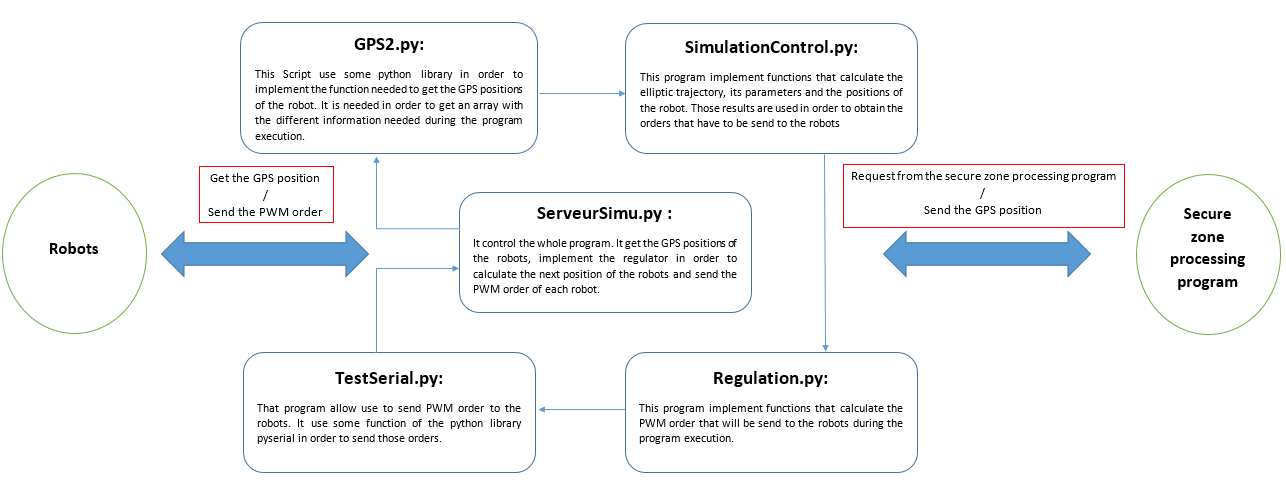
\includegraphics[scale=0.5,angle=90]{SyntheseCodeRegulationRobot.PNG}
    \caption{Architecture of the program which control the regulation of the robots.}
    \label{fig:SyntheseCodeRegulationRobot}
\end{figure}

As you can see, there are 5 main script that are used in order to run the whole program.

For are used in order to implement a part of the functions needed in order to fulfil our purpose:
\begin{itemize}

\item \textbf{GPS2.py}: this script has been implemented by \textcolor{blue}{\textit{Pierre JACQUOT}} and allow us to get access to the GPS signal of all the robots. This program catch the first available GPS tram of each robot, put it in a numpy array. The parameters which are kept are the latitude, the longitude, the speed, the north, the east and the time. The current version allows us to realize a multi-threading program in order to get every GPS positions. In order to call every function, we have to instantiate an object call \textbf{\textit{"ThreadGPSAll"}}
\item SimulationControl.py has been implemented by  \textcolor{blue}{\textit{Alice DANCKAERS}} and is used here in order to get the elliptic trajectory in function of the instant t and the theoretical position of each robots.In order to call every function, we have to instantiate an object call \textbf{\textit{"SimulationControl"}}.
\item Regulation.py has been implemented by  \textcolor{blue}{\textit{Thomas BOULIER and Sylvain HUNAULT}} and is used here in order to get PWM order which have to be send to every robots. Each robots has a PWM in order to go forward and another one in order to turn. It use the theoretical position and the current position of the robot and it return the PWM values. It implement the object \textbf{\textit{"Robot"}} and thanks to it, we are able to keep all the information of the group of robots. Furthermore, it allows us to use the function which are needed in order to regulate every robot. 
\item testserial.py has been implemented by  \textcolor{blue}{\textit{Benoit Raymond }} and is used here in order to send command to every robot. We are using a serial communication in order to send those order to a HF transmitter. Once again, , we have to instantiate an object call \textbf{\textit{"command"}} in order to use the functions in this script.

\end{itemize}

The last one is here in order to organize the whole program and it's called ServeurSimu.py.
It use one thread in order to :
\begin{itemize}
\item Get the current GPS positions of every robots
\item Get the new elliptic trajectory and give the instructions to every robots
\item Get the new PWM command that has to be apply to every robots.
\item Send those PWM instruction. 
\end{itemize}

Whereas, the other thread is here in order to allow a communication between this program and the program which has to run the secure zone processing algorithm.

This script is the master and all the other script are just intermediary in order to regulate the robots. 

\pagebreak